\documentclass[a4paper,ngerman,11pt,bibtotoc]{scrartcl}

\usepackage[utf8]{inputenc}

\usepackage[ngerman]{babel}

\usepackage{amsmath, amsthm, amssymb, stmaryrd, color, graphicx, mathtools, mathrsfs}
\usepackage{setspace}
\usepackage{bussproofs}
\usepackage{array}
\usepackage{booktabs}
\usepackage{comment}
\usepackage{textcomp}
\usepackage{stmaryrd}

\usepackage{tikz}
\usetikzlibrary{shapes,arrows}

\usepackage[protrusion=true,expansion=true]{microtype}

\usepackage{lmodern}
\usepackage{tabto}

\usepackage[backend=bibtex,style=alphabetic]{biblatex}
\usepackage[babel]{csquotes}
\bibliography{literatur}

\usepackage{titling}

\usepackage[all]{xy}

\usepackage[colorlinks=true, linkcolor=blue, urlcolor=blue, citecolor=blue]{hyperref}
\usepackage{cleveref}			%Referenzen mit Name


\usepackage{algorithm}
\usepackage{algpseudocode}
\algrenewcommand{\algorithmiccomment}[1]{\hskip3em$\slash\slash$ #1}
\newcommand{\LineFor}[2]{\State\algorithmicfor\ {#1}\ \algorithmicdo\ {#2} \algorithmicend\ \algorithmicfor}


\setlength\parskip{\medskipamount}
\setlength\parindent{0pt}

\theoremstyle{definition}
\newtheorem{defn}{Definition}[section]
\newtheorem{axiom}[defn]{Axiom}
\newtheorem{bsp}[defn]{Beispiel}

\theoremstyle{plain}

\newtheorem{prop}[defn]{Proposition}
\newtheorem{motto}[defn]{Motto}
\newtheorem{ueberlegung}[defn]{Überlegung}
\newtheorem{lemma}[defn]{Lemma}
\newtheorem{kor}[defn]{Korollar}
\newtheorem{hilfsaussage}[defn]{Hilfsaussage}
\newtheorem{satz}[defn]{Satz}

\theoremstyle{remark}
\newtheorem{erin}[defn]{Erinnerung}
\newtheorem{bem}[defn]{Bemerkung}
\newtheorem{beob}[defn]{Beobachtung}
\newtheorem{aufg}[defn]{Aufgabe}

\clubpenalty=10000
\widowpenalty=10000
\displaywidowpenalty=10000

\newcommand{\IZ}{\mathbb{Z}}
\newcommand{\IQ}{\mathbb{Q}}
\newcommand{\IR}{\mathbb{R}}
\newcommand{\IC}{\mathbb{C}}
\newcommand{\IN}{\mathbb{N}}
\newcommand{\Ic}{\mathcal{I}}
\newcommand{\Jc}{\mathcal{J}}
\newcommand{\Hc}{\mathcal{H}}
\newcommand{\Tc}{\mathcal{T}}
\newcommand{\Sc}{\mathcal{S}}
\newcommand{\Oc}{\mathcal{O}}

% Nur für dieses Dokument %%%%%%%%%%%%%%%%%%%%%%%%%%%%%%%%%%%%%%

\newcommand{\ClientSet}{\mathscr{C}}
\newcommand{\FacilitySet}{\mathscr{F}}
\newcommand{\allTours}{\mathscr{T}}

\newcommand{\OPT}{\mathrm{OPT}}
\newcommand{\CLR}{\mathrm{CLR}}
\newcommand{\CLRHFC}{\mathrm{CLRhFC}}
\newcommand{\MST}{\mathrm{MST}}
\newcommand{\ULF}{\mathrm{ULF}}

% C++ from http://tex.stackexchange.com/a/4304
\def\Cpp{{C\nolinebreak[4]\hspace{-.05em}\raisebox{.4ex}{\tiny\bf ++}}}

\renewcommand*\theenumi{\alph{enumi}}
\renewcommand{\labelenumi}{(\theenumi)}

\setcounter{tocdepth}{2}


\usepackage{todonotes}


% DOCUMENT %%%%%%%%%%%%%%%%%%%%%%%%%%%%%%%%%%%%%%%%%%%%%%%%%%%%%

\begin{document}
\author{Lukas Graf}
\date{Letzte Aktualisierung: \today}

\selectlanguage{ngerman}
\thispagestyle{empty}


\begin{titlepage}\center
	\textsc{\LARGE Universität Augsburg}\\[1cm]
	
	\textsc{\Large Institut für Mathematik}\\[1.5cm]
	
	% Title
	{\Large Ausarbeitung \\[1cm]}
	zum Programmierprojekt\\[1cm]
	{\huge Capacitated Location Routing \\ with Hard Facility Capacities}

	\begin{center}
		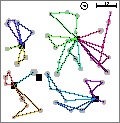
\includegraphics[width=.6\textwidth]{bilder/title.pdf}
	\end{center}		
	
	\vfill
	
	% Author and supervisor
	\begin{minipage}{0.4\textwidth}
		\begin{flushleft} \large
			\emph{von:}\\
			Lukas \textsc{Graf}
		\end{flushleft}
	\end{minipage}
	\begin{minipage}{0.4\textwidth}
		\begin{flushright} \large
			\emph{Betreut von:} \\
			Prof. Dr. Tobias \textsc{Harks}
		\end{flushright}
	\end{minipage}
	
\end{titlepage}

% CONTENT %%%%%%%%%%%%%%%%%%%%%%%%%%%%%%%%%%%%%%%%%%%


\tableofcontents

\newpage
	
\section*{\glqq Abstract\grqq}

\todo[inline]{Zusammenfassung/Überblick der Arbeit}


\section{Capacitated Location Routing (CLR)}

	\subsection{Problemdefinition}

Eine Instanz des \textbf{Capacitated Location Routing Problems (CLR)} ist gegeben durch
\begin{itemize}
	\item einen ungerichteten, zusammenhängenden Graphen $G =(V,E)$,
	\item eine Partition der Knoten in Kunden $\ClientSet$ und Fabrikstandorte $\FacilitySet$,
	\item eine metrischen Kostenfunktion auf den Kanten $c: E \to \IR_{\geq 0}$,
	\item Eröffnungskosten für die Fabriken $\phi: \FacilitySet \to \IR_{\geq 0}$,
	\item Bedarfe der Kunden $d: \ClientSet \to \IR_{\geq 0}$
	\item und eine einheitliche Kapazität $u > 0$ für die Fahrzeuge.		
\end{itemize}
Zulässige Lösungen bestehen aus
\begin{itemize}
	\item einer Teilmenge $F \subseteq \FacilitySet$ von eröffneten Fabriken
	\item und einer Menge von Touren $\Tc = \{T_1, \dots, T_k\}$,
\end{itemize}
sodass gilt:
\begin{itemize}
	\item Zu jeder Tour gibt es eine geöffnete Fabrik $f \in F$, an der diese startet und endet.
	\item Alle Touren zusammen erfüllen alle Bedarfe der Kunden.
	\item Keine der Touren übersteigt die Kapazität $u$.
\end{itemize}
Das Optimierungsziel ist es die Gesamtkosten für das Eröffnen der Fabriken und die gefahrenen Touren zu minimieren, also die Minimierung der Kostenfunktion
\footnote{Wir verwenden hier, dass eine Funktion $\IR$-wertige Funktion $c: M \to \IR$ auf einer Menge $M$ eine Funktion $\tilde{c}: \mathcal{P}(M) \to \IR: M \supseteq N \mapsto \sum_{x \in N} c(x)$ auf der Potenzmenge $\mathcal{P}(M)$ induziert. Zur Vereinfachung der Notation bezeichnen wir diese Funktion dann ebenfalls mit $c$. Unter nochmaliger Anwendung dieser Konvention ließe sich die obige Kostenfunktion daher auch als $c(\Tc) + \phi(F)$ schreiben.}
	\[\sum_{T\in\Tc} c(T) + \sum_{f\in F}\phi(f) \]
	
\begin{beob}
	$\CLR{}$ ist NP-schwer, denn es beinhaltet beispielsweise metrisches TSP (betrachte Instanzen mit $|\FacilitySet| = 1$, $d \equiv 1$ und $u = |\ClientSet|$).
\end{beob}


	\subsection{Ein Approximationsalgorithmus für $\CLR$}

Der in \cite{AAfCLR} beschriebene $4,38$-approximative Algorithmus für $\CLR$ basiert im Wesentlichen auf den folgenden Schritten (schematisch dargestellt in \cref{fig:CLRAlg}):

\todo[inline]{Algorithmus beschreiben (auf schlechtere Approximationsgüte der Implementierung hinweisen!)}


\begin{figure}[H]
	\begin{tiny}
		
\tikzstyle{Absch} = [rectangle, draw, 
    text centered]
\tikzstyle{keinBeweis} = [rectangle, fill=gray!25, 
    text centered]    

\tikzstyle{BewTeil} = []


\tikzstyle{Box} = [rectangle, draw, text centered, rounded corners]
\tikzstyle{Alg} = [rectangle, draw, fill=gray!50, text centered]
\tikzstyle{Text} = [text centered]
\tikzstyle{Image} = []

\tikzstyle{arrow} = [draw, -latex']
\tikzstyle{line} = [draw]


\begin{tikzpicture}[node distance = 5em, auto]

% EINGABE:
\node [Box, text width=20em] (input) {\textbf{Input:} \\ CLR-Instanz $((\ClientSet\cup\FacilitySet,E),c,\phi,d,u)$};
\node [below of=input] (under-input) {};
\node [Image, above of=input, node distance=6em] (input-img) {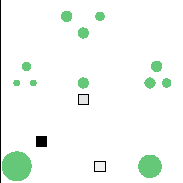
\includegraphics[width=8em]{bilder/instance.pdf}};

% ULF-Instanz:
\node [Box, left of=under-input, text width=14em, node distance=8em] (ULF) 
	{\textbf{ULF-Instanz:} \\ $((\ClientSet\cup\FacilitySet,E),\tilde{c},\phi,d)$ \\
	wobei $\tilde{c}:E \to \IR_{\geq 0}: e \mapsto \frac{2}{u}c(e)$};
\node [Text, left of=ULF, text width=12em, node distance=15em] (ULF-lower-bound) {$\leadsto$ Untere Schranke: $\OPT(\CLR) \geq \OPT(\ULF)$};
\node [Alg, below of=ULF, text width=14em] (ULF-solving) {löse approximativ (mit Greedy)};
\node [Image, left of=ULF-solving, node distance=15em] (ULF-img) {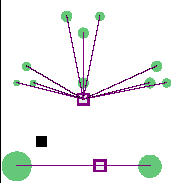
\includegraphics[width=5em]{bilder/ULF.pdf}};

% MST-Instanz:
\node [Box, right of=under-input, text width=14em, node distance=8em] (MST)
	{\textbf{MST-Instanz:} \\ $((\ClientSet\cup\FacilitySet\cup\{r\},E^\prime),c^\prime)$ \\
	$E^\prime := E \cup \{\{r,f\}\mid f\in\FacilitySet\}$ \\
	$c^\prime(f,v) := c(f,v) + \frac{1}{2}\phi(f),$ \\
	$c^\prime(r,f) := 0, c^\prime(v,w):=c(c,w)$};
\node [Text, right of=MST, text width=12em, node distance=15em] (MST-lower-bound) {$\leadsto$ Untere Schranke: $\OPT(\CLR) \geq \OPT(\MST)$};
\node [Alg, below of=MST, text width=14em] (MST-solving) {löse exakt (mit ???)};
\node [Image, right of=MST-solving, node distance=15em] (MST-img) {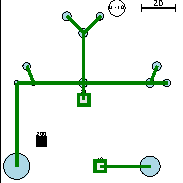
\includegraphics[width=5em]{bilder/MST.pdf}};

% MERGE-Phase:
\node [Text, below of=under-input, node distance=8em] (merge) {\textbf{Merge-Phase:}};

\node [Alg, below of=merge, node distance=1.5em, text width=30em] (m-facilities) {
		\begin{minipage}{30em}\begin{algorithmic}
		\State Eröffne in $\ULF$ oder $\MST$ verwendete Fabriken
		\end{algorithmic}\end{minipage}
	};
\node [Text, left of=m-facilities, node distance=25em, text width=15em] () 
	{beschränkt durch die entsprechenden Eröffnungskosten in $\ULF$ und $\MST$};

% Große Klienten
\node [Alg, below of=m-facilities, node distance=4em] (m-big-clients) {
		\begin{minipage}{30em}\begin{algorithmic}
		\For{Klienten $v$ mit $d(v)\geq u$}
			\State Verbinde $v$ durch $\frac{d(v)}{u}$ Touren mit nächster offener Fabrik
		\EndFor
		\end{algorithmic}\end{minipage}
	};
\node [Image, right of=m-big-clients, node distance=25em] () {
	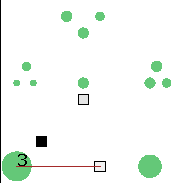
\includegraphics[width=5em]{bilder/largeDemand1.pdf}
	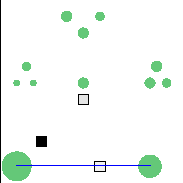
\includegraphics[width=5em]{bilder/largeDemand2.pdf}
};
\node [Text, left of=m-big-clients, node distance=25em, text width=15em] () 
	{beschränkt durch $2\times$ den entsprechenden Verbindungskosten in $\ULF$};

% Kleine Klienten
\node [Alg, below of=m-big-clients, node distance=4em] (m-small-clients) {
		\begin{minipage}{30em}\begin{algorithmic}\algtext*{EndFor}
		\For{Durch $\MST$ eröffnete Fabrik $f$ tue}
		\State Definitionen...
		\EndFor
		\end{algorithmic}\end{minipage}
	};

% Relieve-Schritte
\node [Alg, below of=m-small-clients, node distance=5em] (m-relieve) {
		\begin{minipage}{30em}\begin{algorithmic}\algtext*{For}\algtext*{EndFor}
			\For
			\While{$D_f > 0$}
			\State Finde $v \in S_f$ mit $D_v > u$ und f.a. Kinder $w$ von $v$: $D_w \leq u$
			\State Zerlege $S_v$ in Teilbäume ...
			\EndWhile
			\EndFor
			\end{algorithmic}\end{minipage}
	};
\node [Image, right of=m-relieve, node distance=25em] () {
		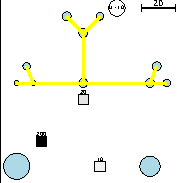
\includegraphics[width=5em]{bilder/relieveTour1.pdf}
		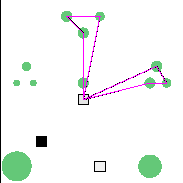
\includegraphics[width=5em]{bilder/relieveTour2.pdf}
		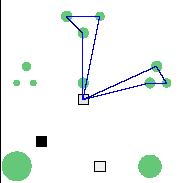
\includegraphics[width=5em]{bilder/relieveTour3.pdf}
	};
\node [Text, left of=m-relieve, node distance=25em, text width=15em] () 
	{Jede Tour ist beschränkt durch $2\times$ die Kantenkosten im $\MST$ und $2\times$ den Verbindungskosten aller Knoten der Tour in $\ULF$};

% Rest
\node [Alg, below of=m-relieve, node distance=5em] (m-remaining) {
		\begin{minipage}{30em}\begin{algorithmic}\algtext*{For}
		\For
		\State Mache Rest
		\EndFor
		\end{algorithmic}\end{minipage}
	};
\node [Image, right of=m-remaining, node distance=25em] () {
	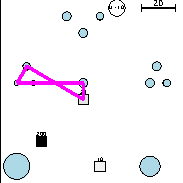
\includegraphics[width=5em]{bilder/remainingTour1.pdf}
	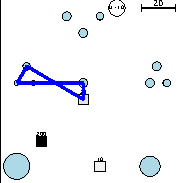
\includegraphics[width=5em]{bilder/remainingTour2.pdf}
};
\node [Text, left of=m-remaining, node distance=25em, text width=15em] () 
	{beschränkt durch $2\times$ den Verbindungskosten in $\MST$};


% AUSGABE:
\node [Box, below of=m-remaining, node distance=3em] (output) {\textbf{Output}};
\node [Image, below of=output] (outpu-img) {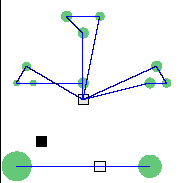
\includegraphics[width=8em]{bilder/output.pdf}};


% PATHS:

\path [arrow] (input.south) -- (ULF.north);    
\path [arrow] (input.south) -- (MST.north); 

\path [arrow] (ULF) -- (ULF-solving.north);
\path [arrow] (MST) -- (MST-solving.north);
\path [arrow] (ULF-solving.south) -- (merge.north);
\path [arrow] (MST-solving.south) -- (merge.north);

\path [line] (m-facilities) -- (m-big-clients);
\path [line] (m-big-clients) -- (m-small-clients);
\path [line] (m-small-clients) -- (m-relieve);
\path [line] (m-relieve) -- (m-remaining);

\path [arrow] (m-remaining.south) -- (output.north);

\end{tikzpicture}

	\end{tiny}
	\caption{Schematische Darstellung des Algorithmus für CLR}\label{fig:CLRAlg}
\end{figure}

\subsection{Visualisierung des Algorithmus}

Im ersten Teil des Programmierprojektes ging es darum den Ablauf sowie das Ergebnis des oben beschriebenen Algorithmus zu visualisieren. Dazu wurde die existierende Implementierung des Algorithmus um eine Klasse \texttt{CLR\_Drawing} erweitert. Diese wird zu Beginn des Algorithmus mit der zu lösenden Instanz initialisiert und kann dann an verschiedenen Stellen des Algorithmus aufgerufen werden, um einen Schnappschuss mit dem momentanen Stand zu erstellen. 

Die Ausgabe besteht aus SVG-Dateien, die mit Hilfe der \Cpp-Bibliothek simple-svg (\cite{simple-svg}) erstellt werden. Diese können dann beispielsweise von Hand übereinander gelegt werden, um ein bestimmtes Zwischenstadium des Algorithmus darzustellen, oder zu einer Animation zusammengesetzt werden, um den gesamten Ablauf des Algorithmus abzubilden. 

\begin{figure}[H]\centering\setlength{\fboxsep}{0pt}
	\fbox{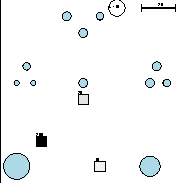
\includegraphics[width=.19\textwidth]{bilder/demo_instance.pdf}}
	\fbox{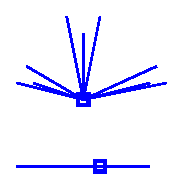
\includegraphics[width=.19\textwidth]{bilder/demo_ULF.pdf}}
	\fbox{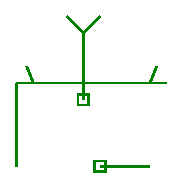
\includegraphics[width=.19\textwidth]{bilder/demo_Tree.pdf}}
	\fbox{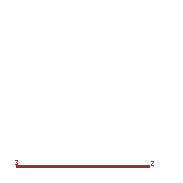
\includegraphics[width=.19\textwidth]{bilder/demo_LargeDemand.pdf}}
	\fbox{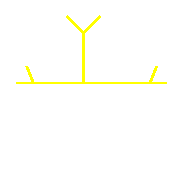
\includegraphics[width=.19\textwidth]{bilder/demo_relieveTree.pdf}}
	
	\fbox{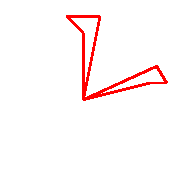
\includegraphics[width=.19\textwidth]{bilder/demo_relieveTour.pdf}}
	\fbox{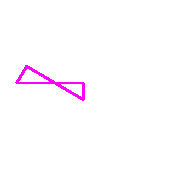
\includegraphics[width=.19\textwidth]{bilder/demo_remainingTour.pdf}}
	\fbox{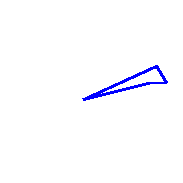
\includegraphics[width=.19\textwidth]{bilder/demo_singleTour.pdf}}
	\fbox{
\includegraphics[width=.19\textwidth]{bilder/demo_allTours.pdf}}
	
	\caption{Ausgabe der Klasse \texttt{CLR\_Drawing}: Die Instanz selbst, die Lösung der ULF-Instanz, die Lösung der MST-Instanz, Touren aus der Large-Demand-Phase, ein Relieve-Tree, eine daraus entstandene Tour, eine Remaining-Tour, eine einzelne Tour, alle Touren}
\end{figure}

Ein Beispiel für ersteres sind die Bilder in dieser Arbeit, als Beispiel für Letztes \todo{Verweis auf Webseite/Anhang/...?}...

\todo[inline]{Klasse detaillierter beschreiben?}

	

\section{$\CLR$ with Hard Facility Capacities ($\CLRHFC$)}

Eine Verallgemeinerung von $\CLR$ erhält man, indem man die Kapazitäten der Fabriken beschränkt. In diesem Kapitel geht es darum, wie der Approximationsalgorithmus für $\CLR$ so angepasst werden kann, dass er auch für das neue Problem zulässige Lösungen findet.

	\subsection{Problemdefinition}

Eine Instanz von \textbf{Capacitated Location Routing with Hard Facility Capacities ($\CLRHFC$)} ist gegeben durch:
\begin{itemize}
	\item eine Instanz $(G=(\ClientSet\cup\FacilitySet,E), c,\phi,d,u)$ von $\CLR$
	\item und zusätzlich Kapazitäten der Fabriken $l: \FacilitySet \to \IR_{\geq 0}$.
\end{itemize}
Zulässige Lösungen sind Lösungen der zugrunde liegenden $\CLR$-Instanz, die zudem die Kapazitätsschranken der Fabriken einhalten.

Das Optimierungsziel ist weiterhin die Minimierung der unveränderten Kostenfunktion der $\CLR$-Instanz.

\begin{bem}
Es gibt auch Varianten von $\CLR$ mit \emph{weichen Fabrikkapazitäten}. 

\todo[inline]{Näher erklären, Quellen (z.B. 10.1007/s00453-007-9032-7 ?)}
\end{bem}

$\CLRHFC$ kann auch wie folgt als Mixed Integer Program (MIP) beschrieben werden:

\begin{center}
	minimiere
	\begin{align*}\sum_{f \in \FacilitySet} o_f \phi(f) + \sum_{T \in \allTours} y_T c(T)\end{align*}
	unter den Nebenbedingungen:
	\begin{align}	\sum_{v \in T\backslash\FacilitySet} x_{vT} \leq u y_T 								&,\quad T \in \allTours 						\\
	\sum_{T \in \allTours_f} \sum_{v \in T\backslash\FacilitySet} x_{vT} \leq o_f l(f)	&,\quad f \in \FacilitySet						\\
	\sum_{T \in \allTours, v \in T} x_{vT} \geq d(v)									&,\quad v \in \ClientSet					
	\end{align}
	wobei
	\begin{align*}o_f \in \{0,1\},\quad y_T \in \IN_0, \quad x_{vT} \geq 0\end{align*}
\end{center}

Dabei gibt es 
\begin{itemize}
	\item für jede Fabrik eine Variable $o_f$, welche bestimmt, ob die entsprechende Fabrik geöffnet ($1$) ist oder nicht ($0$),
	\item sowie für jede mögliche Tour $T$ eine Variabel $y_T$, welche bestimmt, wie oft die entsprechende Tour genutzt wird,
	\item und für jeden auf $T$ liegenden Kunden $v$ eine Variable $x_{vT}$, welche besagt, wie viele Einheiten durch Tour $T$ insgesamt an den Kunden $v$ geliefert werden.
\end{itemize}

Die Nebenbedingungen bekommen damit die folgende Bedeutung:
\begin{enumerate}\renewcommand{\theenumi}{\arabic{enumi}}
	\item Die Fahrzeugkapazität ($u$) wird eingehalten. D.h. wird eine Tour $y_T$-mal genutzt, so können durch sie höchstens $y_T u$ Einheiten an die auf ihr liegenden Kunden geliefert werden.
	\item Die Fabrikkapazitäten ($l$) werden eingehalten. Alle bei eine Fabrik $f$ beginnenden Touren ($\allTours_f$) können zusammen höchstens so viele Einheiten ausliefern, wie die Fabrikkapazität $l(f)$ zulässt.
	\item Die Bedarfe der Kunden ($d$) werden erfüllt. Dies ist der Fall, wenn alle Touren, auf denen ein Kunde $v$ liegt, zusammen mindestens so viel an ihn liefern, wie sein Bedarf $d(v)$ ist.
\end{enumerate}

\begin{beob}
	Die Menge aller denkbaren Touren $\allTours$ wächst exponentiell in der Zahl der Kunden der $\CLRHFC$-Instanz. Dementsprechend schnell steigt auch die Zahl der Variablen und der Nebenbedingungen an, sodass das Problem nur für sehr kleine Eingabeinstanzen exakt gelöst werden kann.
\end{beob}


	\subsection{Lösungsansätze}
	
	Um überhaupt zulässige Lösungen für $\CLRHFC$ zu finden, muss der bestehende Algorithmus an wenigstens zwei Stellen angepasst werden: Beim Erstellen der Touren muss nun zusätzlich darauf geachtet werden, dass die Kapazität der ausgewählten Fabrik nicht überschritten wird. Und allgemein muss immer gewährleistet sein, dass überhaupt offene Fabriken mit freier Kapazität verfügbar sind.
	
	Ersteres lässt sich sicherstellen, indem Touren gegebenenfalls noch weiter in Teiltouren aufgespalten werden, die jeweils klein genug sind, um von einer einzelnen offenen Fabrik vollständig beliefert zu werden.
	
	Für Letzteres gibt es zwei naheliegende Ansätze: Entweder man passt die $\ULF$- und/oder $\MST$-Phase so an, dass bereits hier die Fabrikkapazitäten berücksichtigt und dementsprechend viele Fabriken geöffnet werden. Oder man erlaubt dem Algorithmus zusätzlich noch in der Large-Demand- bzw. Merge-Phase bei Bedarf weiter Fabriken zu eröffnen. 
	
	Der erste Ansatz ließe sich beispielsweise dadurch verwirklichen, dass statt einer $\ULF$-Instanz eine Instanz des \emph{nonuniform Capacitated Facility Location Problem}s erstellt und (approximativ) gelöst wird. Ein entsprechender auf lokaler Suche basierender Approximationsalgorithmus wird in \cite{Pal01facilitylocation} beschrieben. Alternativ (oder auch zusätzlich) könnte man versuchen beim Erstellen des Spannbaumes die Fabrikkapazitäten zu berücksichtigen. Dies hätte möglicherweise den Vorteil \todo{Add Vorteil}. Allerdings ist nicht klar, wie eine entsprechende Anpassung dieser Phase aussehen könnte.
	
	Der zweite Ansatz - neue Fabriken bei Bedarf eröffnen - ist dagegen deutlich leichter zu implementieren und ist daher auch der, der in diesem Programmierprojekt weiterverfolgt wurde. Er hat allerdings den Nachteil, dass dadurch der Zusammenhang zwischen den Kosten der in $\ULF$- und $\MST$-Phase gefundenen Lösungen und denen der letztendlich bestimmten Lösung der $\CLRHFC$-Instanz verloren gehen. \todo{siehe \cref{sec:Analyse}}

	\subsection{Der Algorithmus und seine Implementierung}
	
\todo[inline]{Allgemeines zur Implementierungsphilosophie (Vererbung)}		
\todo[inline]{Beschreibung des angepassten Algorithmus}

	\subsubsection{Toursplitting}

	\subsubsection{Greedy Fabrikeröffnung}
	
	\subsubsection{Fabrikeröffnung durch wiederholtes $\ULF$/$\MST$}
	
	\subsubsection{Zulässigkeitsprüfung}
	
	\begin{figure}[H]
	\tikzstyle{vertex} = [circle,draw]
	\tikzstyle{edge} = [draw]
	\tikzstyle{beschr} = []
	\tikzstyle{beschrR} = [text width=25em]
	\begin{tikzpicture}[->,>=stealth',shorten >=1pt,auto,node distance=6em,thick]
	
	\node[vertex] (quelle) {Quelle};
		\node[beschr, left of=quelle, node distance=15em](bQuelle) {};
		\node[beschrR, right of=quelle, node distance=25em](bRQuelle) {};
	
	\node[below of=quelle] (fs) {$\dots$};		
		\node[beschr, below of=bQuelle](bFs) {Fabriken:};
		\node[beschrR, below of=bRQuelle, node distance=8.5em](bRFs) {verbinde $f$ mit $T$, \\ falls $T$ bei $f$ beginnt};
	\node[vertex, left of=fs] (f1) {$f_1$};
	\node[vertex, right of=fs] (fm) {$f_m$};
	
	\node[below of=f1] (T1) {$\dots$};
		\node[beschr, below of=bFs](bTs) {Touren:};
		\node[beschrR, below of=bRFs, node distance=7em](bRTs) {verbinde $T$ mit $v$, \\ falls $v$ auf $T$ liegt};
	\node[vertex, left of=T1, node distance=2.5em] (T11) {$T_{11}$};
	\node[vertex, right of=T1, node distance=2.5em] (T1k) {$T_{1k_1}$};

	\node[below of=fm] (Tm) {$\dots$};
	\node[vertex, left of=Tm, node distance=2.5em] (Tm1) {$T_{m1}$};
	\node[vertex, right of=Tm, node distance=2.5em] (Tmk) {$T_{mk_m}$};	
	
	\node[below of=fs] (Ts) {};
	\node[below of=Ts] (vs) {$\dots$};
		\node[beschr, below of=bTs](bVs) {Kunden:};
	\node[vertex, left of=vs] (v1) {$v_1$};
	\node[vertex, right of=vs] (vn) {$v_n$};
	
	\node[vertex, below of=vs] (senke) {Senke};
	
	
	\path[edge] (quelle) to node[left] {$l(f_1)$} (f1);
	\path[edge] (quelle) to node[right] {$l(f_m)$} (fm);
	
	\path[edge] (f1) to node[left] {$u$} (T11);
	\path[edge] (f1) to node[right] {$u$} (T1k);
	\path[edge] (fm) to node[left] {$u$} (Tm1);
	\path[edge] (fm) to node[right] {$u$} (Tmk);
	
	\path[edge] (T11) to node[left] {$u$} (v1);
	\path[edge] (T1k) to node[left] {$u$} (v1);
	\path[edge] (T1k) to node[right] {$u$} (vn);
	\path[edge] (Tm1) to node[left] {$u$} (v1);
	\path[edge] (Tm1) to node[right] {$u$} (vn);
	\path[edge] (Tmk) to node[right] {$u$} (vn);
	
	\path[edge] (v1) to node[left] {$d(v_1)$} (senke);
	\path[edge] (vn) to node[right] {$d(v_n)$} (senke);	
	
	\end{tikzpicture}
	\caption{Die MaxFlow-Instanz \todo[inline]{genauere Beschreibung}}\label{fig:MaxFlowGraph}
	\end{figure}
	
	\todo[inline]{Beschreibe Edmonds-Karp-Implementierung}
	

	\subsection{Analyse der Algorithmen}\label{sec:Analyse}
	
	\subsubsection{Theoretische Betrachtungen}
	
	In \cite{AAfCLR} werden zwei untere Schranken für die Kosten der optimalen $\CLR$-Lösung gezeigt: Die Kosten der optimalen Lösungen der im Algorithmus verwendeten $\ULF$-Instanz sowie die der $\MST$-Instanz. Da jede Lösung einer $\CLRHFC$-Instanz insbesondere auch eine zulässige Lösung der zugrunde liegenden $\CLR$-Instanz sind, gelten diese Schranken weiterhin.
	
	

		\todo[inline]{Untere Schranken}
		
		\todo[inline]{Schlechte Beispiele}
		
	\subsubsection{Heuristische Beurteilung}
	
	 Schon für nur \todo{7?} Kunden und \todo{5?} Fabriken besteht das erzeugte MIP aus \todo{Zahlen einfügen} Variablen und Nebenbedingungen.

	Um das MIP zumindest ein wenig kleiner zu halten, wird bei der Generierung des MIP nicht jede mögliche Tour betrachtet, sondern zu jeder Menge von Kunden und jeder Startfabrik eine jeweils optimale Tour. Zur Lösung des entsprechenden TSPs wird ein sehr einfacher Branch-and-Bound-Algorithmus verwendet. 
	
	


	\subsection{Ausblick}
	
	\todo[inline]{Was könnte man verbessern? Welche Probleme gibt es dabei?}
	
	

\newpage	
\listoftodos

\newpage
\nocite{*}
\printbibliography		
			
\end{document}